% hitex-deck-style: 2
\documentclass[aspectratio=169,11pt]{beamer}
\graphicspath{{../}}
\usetheme{default}
\usepackage{graphicx}
\usepackage{amsmath}
\usepackage{amssymb}
\usepackage{booktabs}
\usepackage{tikz}
\definecolor{hxStructure}{HTML}{37474F}
\definecolor{hxAccent}{HTML}{00796B}
\definecolor{hxMuted}{HTML}{65717A}
\definecolor{hxText}{HTML}{1F2328}
\definecolor{hxBackground}{HTML}{FFFFFF}
\definecolor{hxTitleBg}{HTML}{F4F6F7}
\definecolor{hxTitleFg}{HTML}{37474F}
\definecolor{hxRule}{HTML}{CDD1D3}
\definecolor{hxTint}{HTML}{ABB2B5}
\setbeamercolor{normal text}{fg=hxText,bg=hxBackground}
\setbeamercolor{background canvas}{bg=hxBackground}
\setbeamercolor{structure}{fg=hxStructure}
\setbeamercolor{title}{fg=hxStructure}
\setbeamercolor{frametitle}{fg=hxStructure}
\setbeamercolor{subtitle}{fg=hxMuted}
\setbeamercolor{author}{fg=hxText}
\setbeamercolor{alerted text}{fg=hxAccent}
\setbeamercolor{page number in head/foot}{fg=hxMuted}
\setbeamercolor{itemize item}{fg=hxStructure}
\setbeamercolor{itemize subitem}{fg=hxMuted}
\setbeamerfont{title}{series=\bfseries}
\setbeamerfont{frametitle}{series=\bfseries}
\setbeamertemplate{navigation symbols}{}
\setbeamertemplate{itemize item}{\raisebox{0.12em}{\rule{0.4em}{0.4em}}}
\setbeamertemplate{itemize subitem}{\textendash}
\makeatletter
\newcommand{\hxframes}{18}
% n / N: the total from the last run, or this deck's own count before there is one
\newcommand{\hxtotal}{\ifnum\inserttotalframenumber<\insertframenumber\relax\hxframes\else\inserttotalframenumber\fi}
\setbeamertemplate{frametitle}{%
  \vskip0.45cm%
  \begin{beamercolorbox}[wd=\paperwidth,leftskip=1cm,rightskip=1cm plus 1fil,sep=0pt]{frametitle}%
    \usebeamerfont{frametitle}\insertframetitle\par
    \ifx\insertframesubtitle\@empty\else{\small\color{hxMuted}\insertframesubtitle\par}\fi
    \nointerlineskip\vskip5pt{\color{hxAccent}\rule{1.2cm}{2.5pt}}\par
  \end{beamercolorbox}}
\setbeamertemplate{footline}{%
  \hbox to \paperwidth{\hskip1cm{\color{hxRule}\rule{\dimexpr\paperwidth-2cm\relax}{0.4pt}}\hss}%
  \vskip3pt%
  \hbox to \paperwidth{\hskip1cm\usebeamerfont{page number in head/foot}\usebeamercolor[fg]{page number in head/foot}%
    \insertshorttitle\hfill\insertframenumber\,/\,\hxtotal\hskip1cm}%
  \vskip6pt}
% Title, section and closing slides: a plain frame whose page background is drawn once by \hx@bg.
\let\hx@bg\@empty
\setbeamertemplate{background}{\ifx\hx@bg\@empty\else\hx@bg\global\let\hx@bg\@empty\fi}
% The title and closing slides: the title art (title-art.jpg, next to this file) full-bleed, its left
% side already the title background, and the text set on it on the left.
\newcommand*{\hxpresenter}{}
\newcommand*{\hxcoauthors}{}
\newcommand{\hx@art}[1]{%
  \IfFileExists{title-art.jpg}%
    {\node[anchor=south west,inner sep=0] at (0,0) {
\includegraphics[width=\paperwidth,height=\paperheight]{title-art.jpg}};}%
    {\fill[hxTitleBg] (0,0) rectangle (\paperwidth,\paperheight);}%
  \ifnum#1=1 \fill[hxTitleBg,opacity=0.3] (0,0) rectangle (\paperwidth,\paperheight);\fi}
% Fitting: the title block hangs from 1.2 cm below the top, the author block stands on 0.9 cm above the
% bottom, with at least 0.6 cm (and the accent rule) between them. Measured in saveboxes in one pass;
% when they do not fit: affiliations \tiny, then co-authors \footnotesize, then the title block scaled
% (down to 60 %), then the whole stack scaled.
\newsavebox\hx@titlebox
\newsavebox\hx@authbox
\newdimen\hx@colw
\newdimen\hx@avail
\newdimen\hx@th
\newdimen\hx@ah
\newcommand{\hx@nohyph}{\hyphenpenalty=10000\exhyphenpenalty=10000\raggedright}
\newcommand{\hx@buildtitle}[2]{% #1 title, #2 subtitle (may be empty)
  \sbox\hx@titlebox{\parbox[t]{\hx@colw}{\hx@nohyph
    {\color{hxTitleFg}\huge\bfseries #1\par}%
    \ifx#2\@empty\else\vskip6pt{\color{hxText}\large\bfseries #2\par}\fi}}%
  \hx@th=\ht\hx@titlebox \advance\hx@th by \dp\hx@titlebox}
\newcommand{\hx@buildauthors}[2]{% #1 co-author size, #2 affiliation size
  \sbox\hx@authbox{\parbox[b]{\hx@colw}{\hx@nohyph\color{hxText}%
    {\bfseries\hxpresenter\par}%
    \ifx\hxcoauthors\@empty\else\vskip2pt{#1\hxcoauthors\par}\fi
    \ifx\insertinstitute\@empty\else\vskip4pt{#2\color{hxMuted}\insertinstitute\par}\fi}}%
  \hx@ah=\ht\hx@authbox \advance\hx@ah by \dp\hx@authbox}
\newcommand{\hx@fits}{\dimexpr\hx@th+\hx@ah\relax<\hx@avail}
\newcommand{\hxtitleslide}{\gdef\hx@bg{%
  \hx@colw=0.6\paperwidth
  \hx@avail=\paperheight \advance\hx@avail by -2.7cm \advance\hx@avail by -8.5pt
  \hx@buildtitle{\inserttitle}{\insertsubtitle}%
  \hx@buildauthors{\small}{\scriptsize}%
  \ifdim\hx@fits\else\hx@buildauthors{\small}{\tiny}\fi
  \ifdim\hx@fits\else\hx@buildauthors{\footnotesize}{\tiny}\fi
  \gdef\hx@ts{1}\gdef\hx@as{1}%
  \ifdim\hx@fits\else
    \pgfmathsetmacro\hx@ts{max(0.6,(\hx@avail-\hx@ah)/max(\hx@th,1pt))}%
    \pgfmathparse{(\hx@ts*\hx@th+\hx@ah) > \hx@avail ? 1 : 0}%
    \ifnum\pgfmathresult>0
      \pgfmathsetmacro\hx@as{\hx@avail/(0.6*\hx@th+\hx@ah)}%
      \pgfmathsetmacro\hx@ts{0.6*\hx@as}%
    \fi
  \fi
  \begin{tikzpicture}
  \useasboundingbox (0,0) rectangle (\paperwidth,\paperheight);
  \hx@art{0}
  \node[anchor=north west,inner sep=0] at (1cm,\paperheight-1.2cm) {\scalebox{\hx@ts}{\usebox\hx@titlebox}};
  \node[anchor=south west,inner sep=0] (hxauthors) at (1cm,0.9cm) {\scalebox{\hx@as}{\usebox\hx@authbox}};
  \fill[hxAccent] ([yshift=7pt]hxauthors.north west) rectangle +(1.2cm,1.5pt);
  \end{tikzpicture}}}
\newcommand{\hxclosingslide}[2]{\gdef\hx@bg{%
  \hx@colw=0.6\paperwidth
  \hx@avail=\paperheight \advance\hx@avail by -2.1cm
  \sbox\hx@titlebox{\parbox[t]{\hx@colw}{\hx@nohyph
    {\color{hxTitleFg}\huge\bfseries #1\par}\vskip9pt{\color{hxAccent}\rule{1.2cm}{1.5pt}}\par\vskip6pt
    {\color{hxText}\large #2\par}}}%
  \hx@th=\ht\hx@titlebox \advance\hx@th by \dp\hx@titlebox
  \gdef\hx@ts{1}%
  \ifdim\hx@th>\hx@avail \pgfmathsetmacro\hx@ts{\hx@avail/\hx@th}\fi
  \begin{tikzpicture}
  \useasboundingbox (0,0) rectangle (\paperwidth,\paperheight);
  \hx@art{1}
  % the block's top at 24 % of the height, raised (to 1.2 cm) and then scaled when it is taller
  \pgfmathsetmacro\hx@top{min(0.24*\paperheight, max(1.2cm, \paperheight-0.9cm-\hx@ts*\hx@th))}%
  \node[anchor=north west,inner sep=0] at (1cm,\paperheight-\hx@top pt) {\scalebox{\hx@ts}{\usebox\hx@titlebox}};
  \end{tikzpicture}}}
\newcommand{\hxsectionslide}[2]{\gdef\hx@bg{%
  \begin{tikzpicture}
  \useasboundingbox (0,0) rectangle (\paperwidth,\paperheight);
  \fill[hxStructure] (0,0) rectangle (0.3cm,\paperheight);
  \node[anchor=south west,inner sep=0,text=hxTint] at (1.6cm,0.5\paperheight+0.1cm)
    {\scalebox{2.2}{\Huge\bfseries #1}};
  \node[anchor=north west,inner sep=0,text width=\paperwidth-3.2cm,align=left,text=hxStructure]
    at (1.6cm,0.5\paperheight-0.25cm) {\hyphenpenalty=10000\exhyphenpenalty=10000\LARGE\bfseries #2\par};
  \end{tikzpicture}}}
\makeatother

\title[Benchmarking Single-Cell Forecasting Under Cell Pairings]{Benchmarking Single-Cell Forecasting Under Cell Pairings}
\subtitle{How coupling and evaluation determine what benchmarks can detect}
\author{Victor Ikenna Kanu, Ihunanya Udodiri Ajakwe, Josiah Ayoola Isong, Simeon Okechukwu Ajakwe, Dong-Seong Kim}
\institute{Kumoh National Institute of Technology, Gumi, South Korea\\Kyungdong University Global Campus, South Korea}
\renewcommand*{\hxpresenter}{Victor Ikenna Kanu}
\renewcommand*{\hxcoauthors}{Ihunanya Udodiri Ajakwe, Josiah Ayoola Isong, Simeon Okechukwu Ajakwe, Dong-Seong Kim}
\date{}

\begin{document}

\begin{frame}[plain]
\hxtitleslide
\end{frame}

\begin{frame}{Outline}
\large
\textcolor{hxAccent}{\textbf{01}}\hspace{0.8em}\textcolor{hxStructure}{Motivation}\par\medskip
\textcolor{hxAccent}{\textbf{02}}\hspace{0.8em}\textcolor{hxStructure}{Problem}\par\medskip
\textcolor{hxAccent}{\textbf{03}}\hspace{0.8em}\textcolor{hxStructure}{Approach}\par\medskip
\textcolor{hxAccent}{\textbf{04}}\hspace{0.8em}\textcolor{hxStructure}{Results}\par\medskip
\textcolor{hxAccent}{\textbf{05}}\hspace{0.8em}\textcolor{hxStructure}{Takeaways}\par\medskip
\end{frame}

\section{Motivation}
\begin{frame}[plain]
\hxsectionslide{01}{Motivation}
\end{frame}

\begin{frame}{Can We Forecast Cell States?}
\begin{itemize}
\setlength{\itemsep}{0.6em}
\item{} Predict later differentiation states from earlier single-cell snapshots
\item{} Compare Transformer, random forest, linear, and mechanistic models
\item{} Test whether model capacity improves forecasting
\end{itemize}
\note{Single-cell studies increasingly aim to forecast future differentiation states rather than only describe them. This creates an important comparison question: does a more expressive model actually provide better forecasts? We test that question under a common evaluation protocol.}
\end{frame}

\begin{frame}{The Benchmark Defines the Signal}
\begin{itemize}
\setlength{\itemsep}{0.6em}
\item{} Measurements are destructive across timepoints
\item{} Cells must be linked computationally
\item{} Coupling determines temporal information available to models
\item{} Independent pairing contains no within-trajectory dependence
\end{itemize}
\note{Because standard single-cell measurements are destructive, the same cell is not observed at multiple stages. A benchmark therefore has to construct links between snapshots. Those links are not a technical detail: they determine whether the input contains information about the target.}
\end{frame}

\section{Problem}
\begin{frame}[plain]
\hxsectionslide{02}{Problem}
\end{frame}

\begin{frame}{Independent Pairing Is a Null}
\begin{itemize}
\setlength{\itemsep}{0.6em}
\item{} One independently sampled cell per stage
\item{} Stage order is imposed, not observed
\item{} Late state is independent of earlier states
\item{} Optimal forecast: a constant
\end{itemize}
\note{The main benchmark samples one cell independently at each stage and concatenates the states in stage order. This produces a population-level pseudo-trajectory, not a tracked lineage. Under this construction, the late state is independent of the earlier states, so no model can use the inputs to improve the forecast.}
\end{frame}

\begin{frame}{Evaluation Can Reverse the Verdict}
\begin{columns}[c]
\begin{column}{0.56\textwidth}
\centering
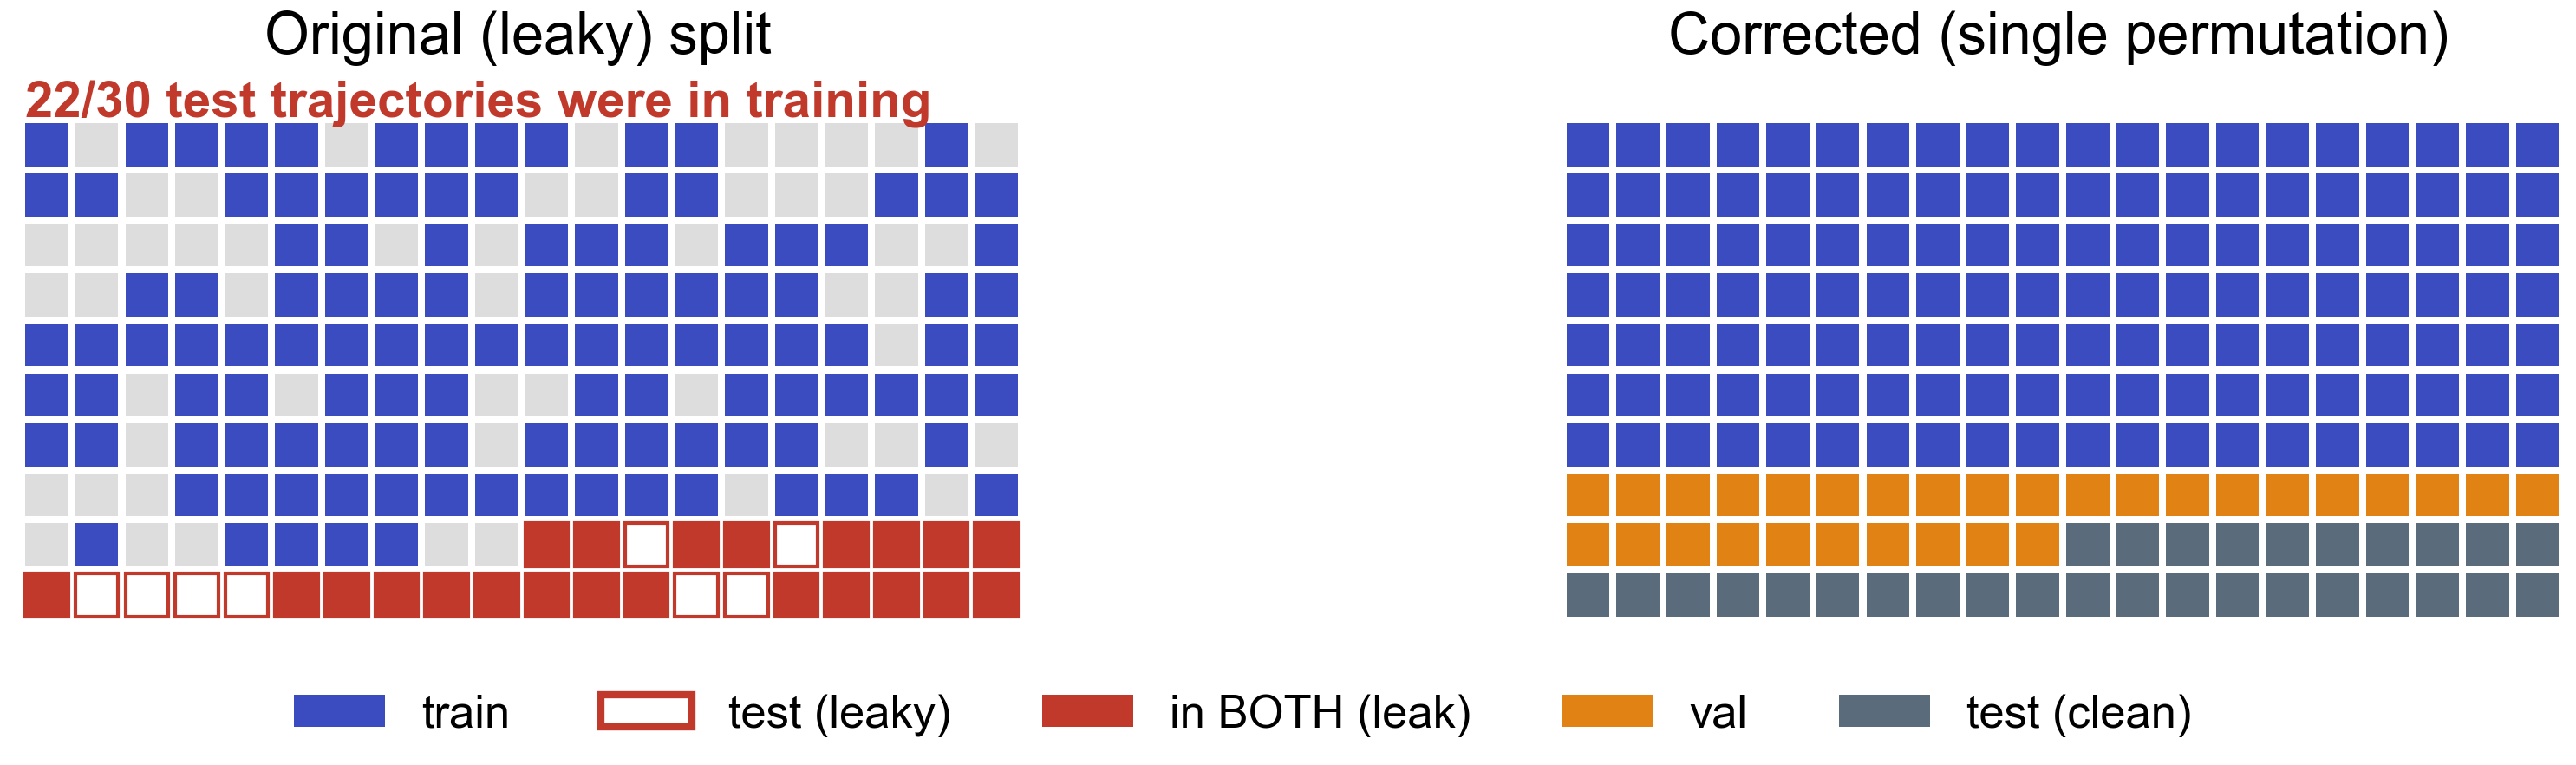
\includegraphics[width=\linewidth,height=0.78\textheight,keepaspectratio]{figures/fig1_leakage_panel.png}
\end{column}
\begin{column}{0.41\textwidth}
\small
\begin{itemize}
\setlength{\itemsep}{0.6em}
\item{} Single-seed comparisons are vulnerable to sampling variation
\item{} Preprocessing before splitting creates leakage
\item{} Earlier pipeline reported a 19.4\% Transformer advantage
\item{} Corrected evaluation reversed that conclusion
\end{itemize}
\end{column}
\end{columns}
\note{The second problem is evaluation rigor. A single seed cannot separate a model difference from trajectory and training randomness, and preprocessing or split inconsistencies can leak information. In this benchmark, the earlier 19.4\% Transformer advantage came from train--test leakage and disappeared under the corrected split.}
\end{frame}

\section{Approach}
\begin{frame}[plain]
\hxsectionslide{03}{Approach}
\end{frame}

\begin{frame}{One Shared, Leakage-Safe Protocol}
\begin{columns}[c]
\begin{column}{0.56\textwidth}
\centering
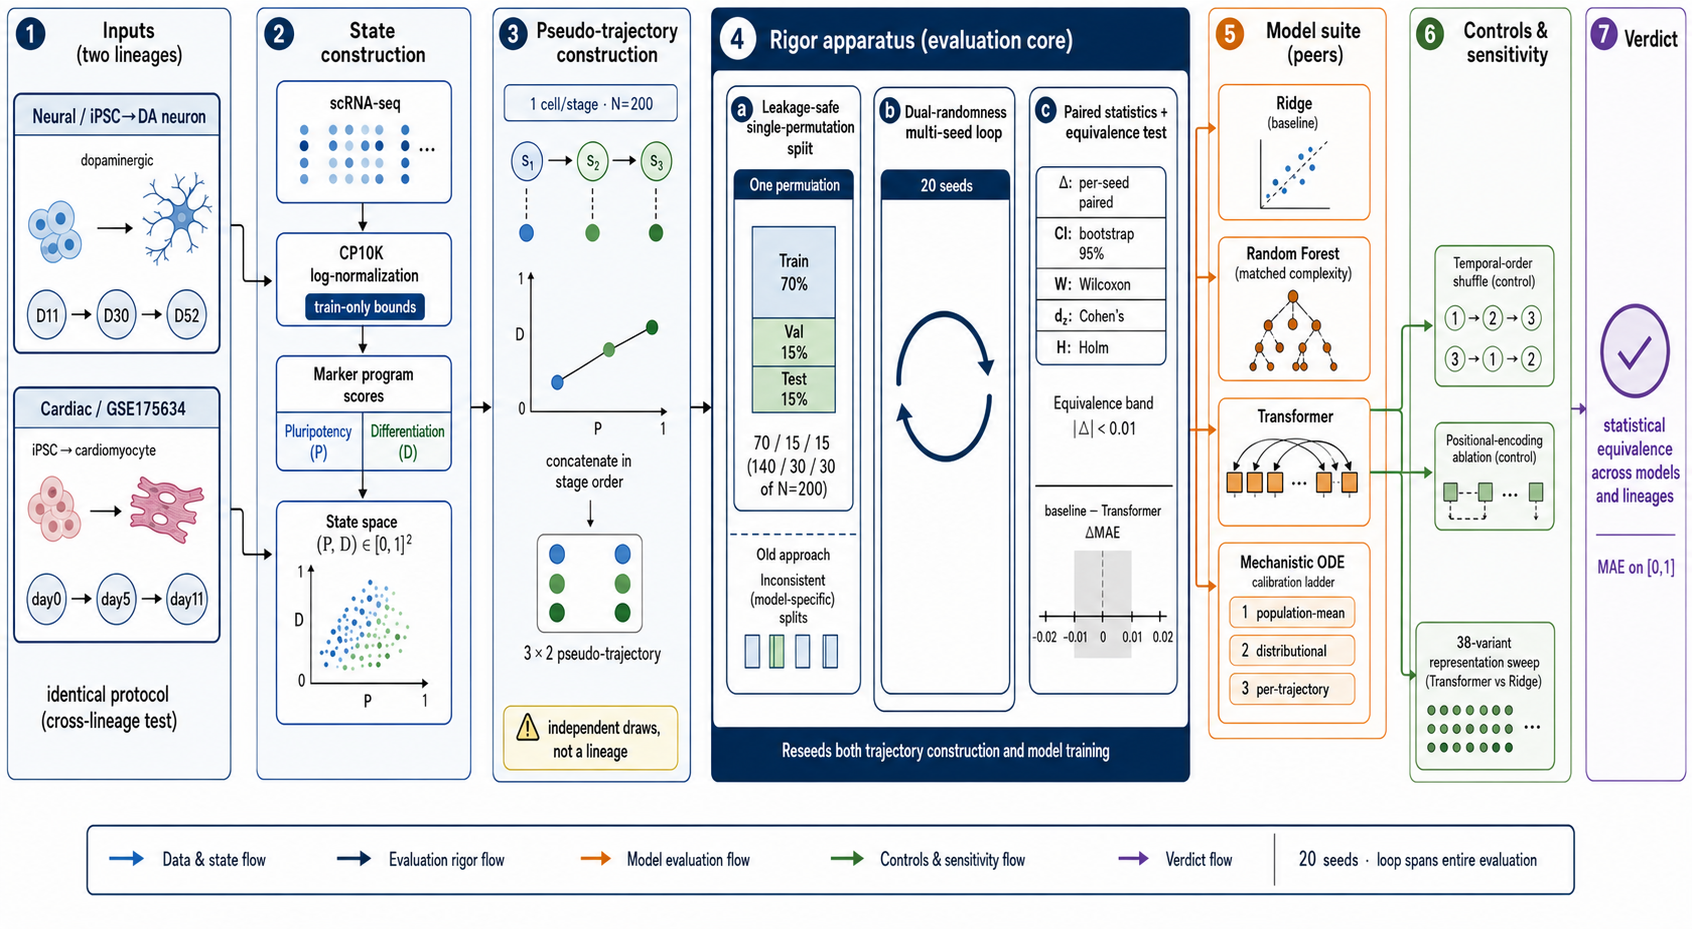
\includegraphics[width=\linewidth,height=0.78\textheight,keepaspectratio]{figures/method_design.png}
\end{column}
\begin{column}{0.41\textwidth}
\small
\begin{itemize}
\setlength{\itemsep}{0.6em}
\item{} Two differentiation lineages and a two-dimensional state
\item{} Shared 70/15/15 split across all models
\item{} Twenty seeds reseed sampling and training
\end{itemize}
\end{column}
\end{columns}
\note{We apply one protocol to neural and cardiac differentiation data. Each cell is represented by pluripotency and lineage-differentiation scores, and 200 pseudo-trajectories are constructed per seed. Every model uses the same split, training-only normalization, and repeated seeds.}
\end{frame}

\begin{frame}{Controls With Known Answers}
\begin{itemize}
\setlength{\itemsep}{0.6em}
\item{} Input-independent training median baseline
\item{} Paired effect sizes and explicit equivalence margin
\item{} Temporal-order and positional-encoding controls
\item{} Simulation and optimal-transport positive controls
\end{itemize}
\note{The protocol includes a constant training-median baseline matched to the MAE evaluation metric. Comparisons use paired statistics over seeds and an equivalence margin of 0.01. We also test temporal controls and positive controls where dependence is known or deliberately induced.}
\end{frame}

\section{Results}
\begin{frame}[plain]
\hxsectionslide{04}{Results}
\end{frame}

\begin{frame}{No Trained Model Beats the Constant}
\begin{columns}[c]
\begin{column}{0.56\textwidth}
\centering
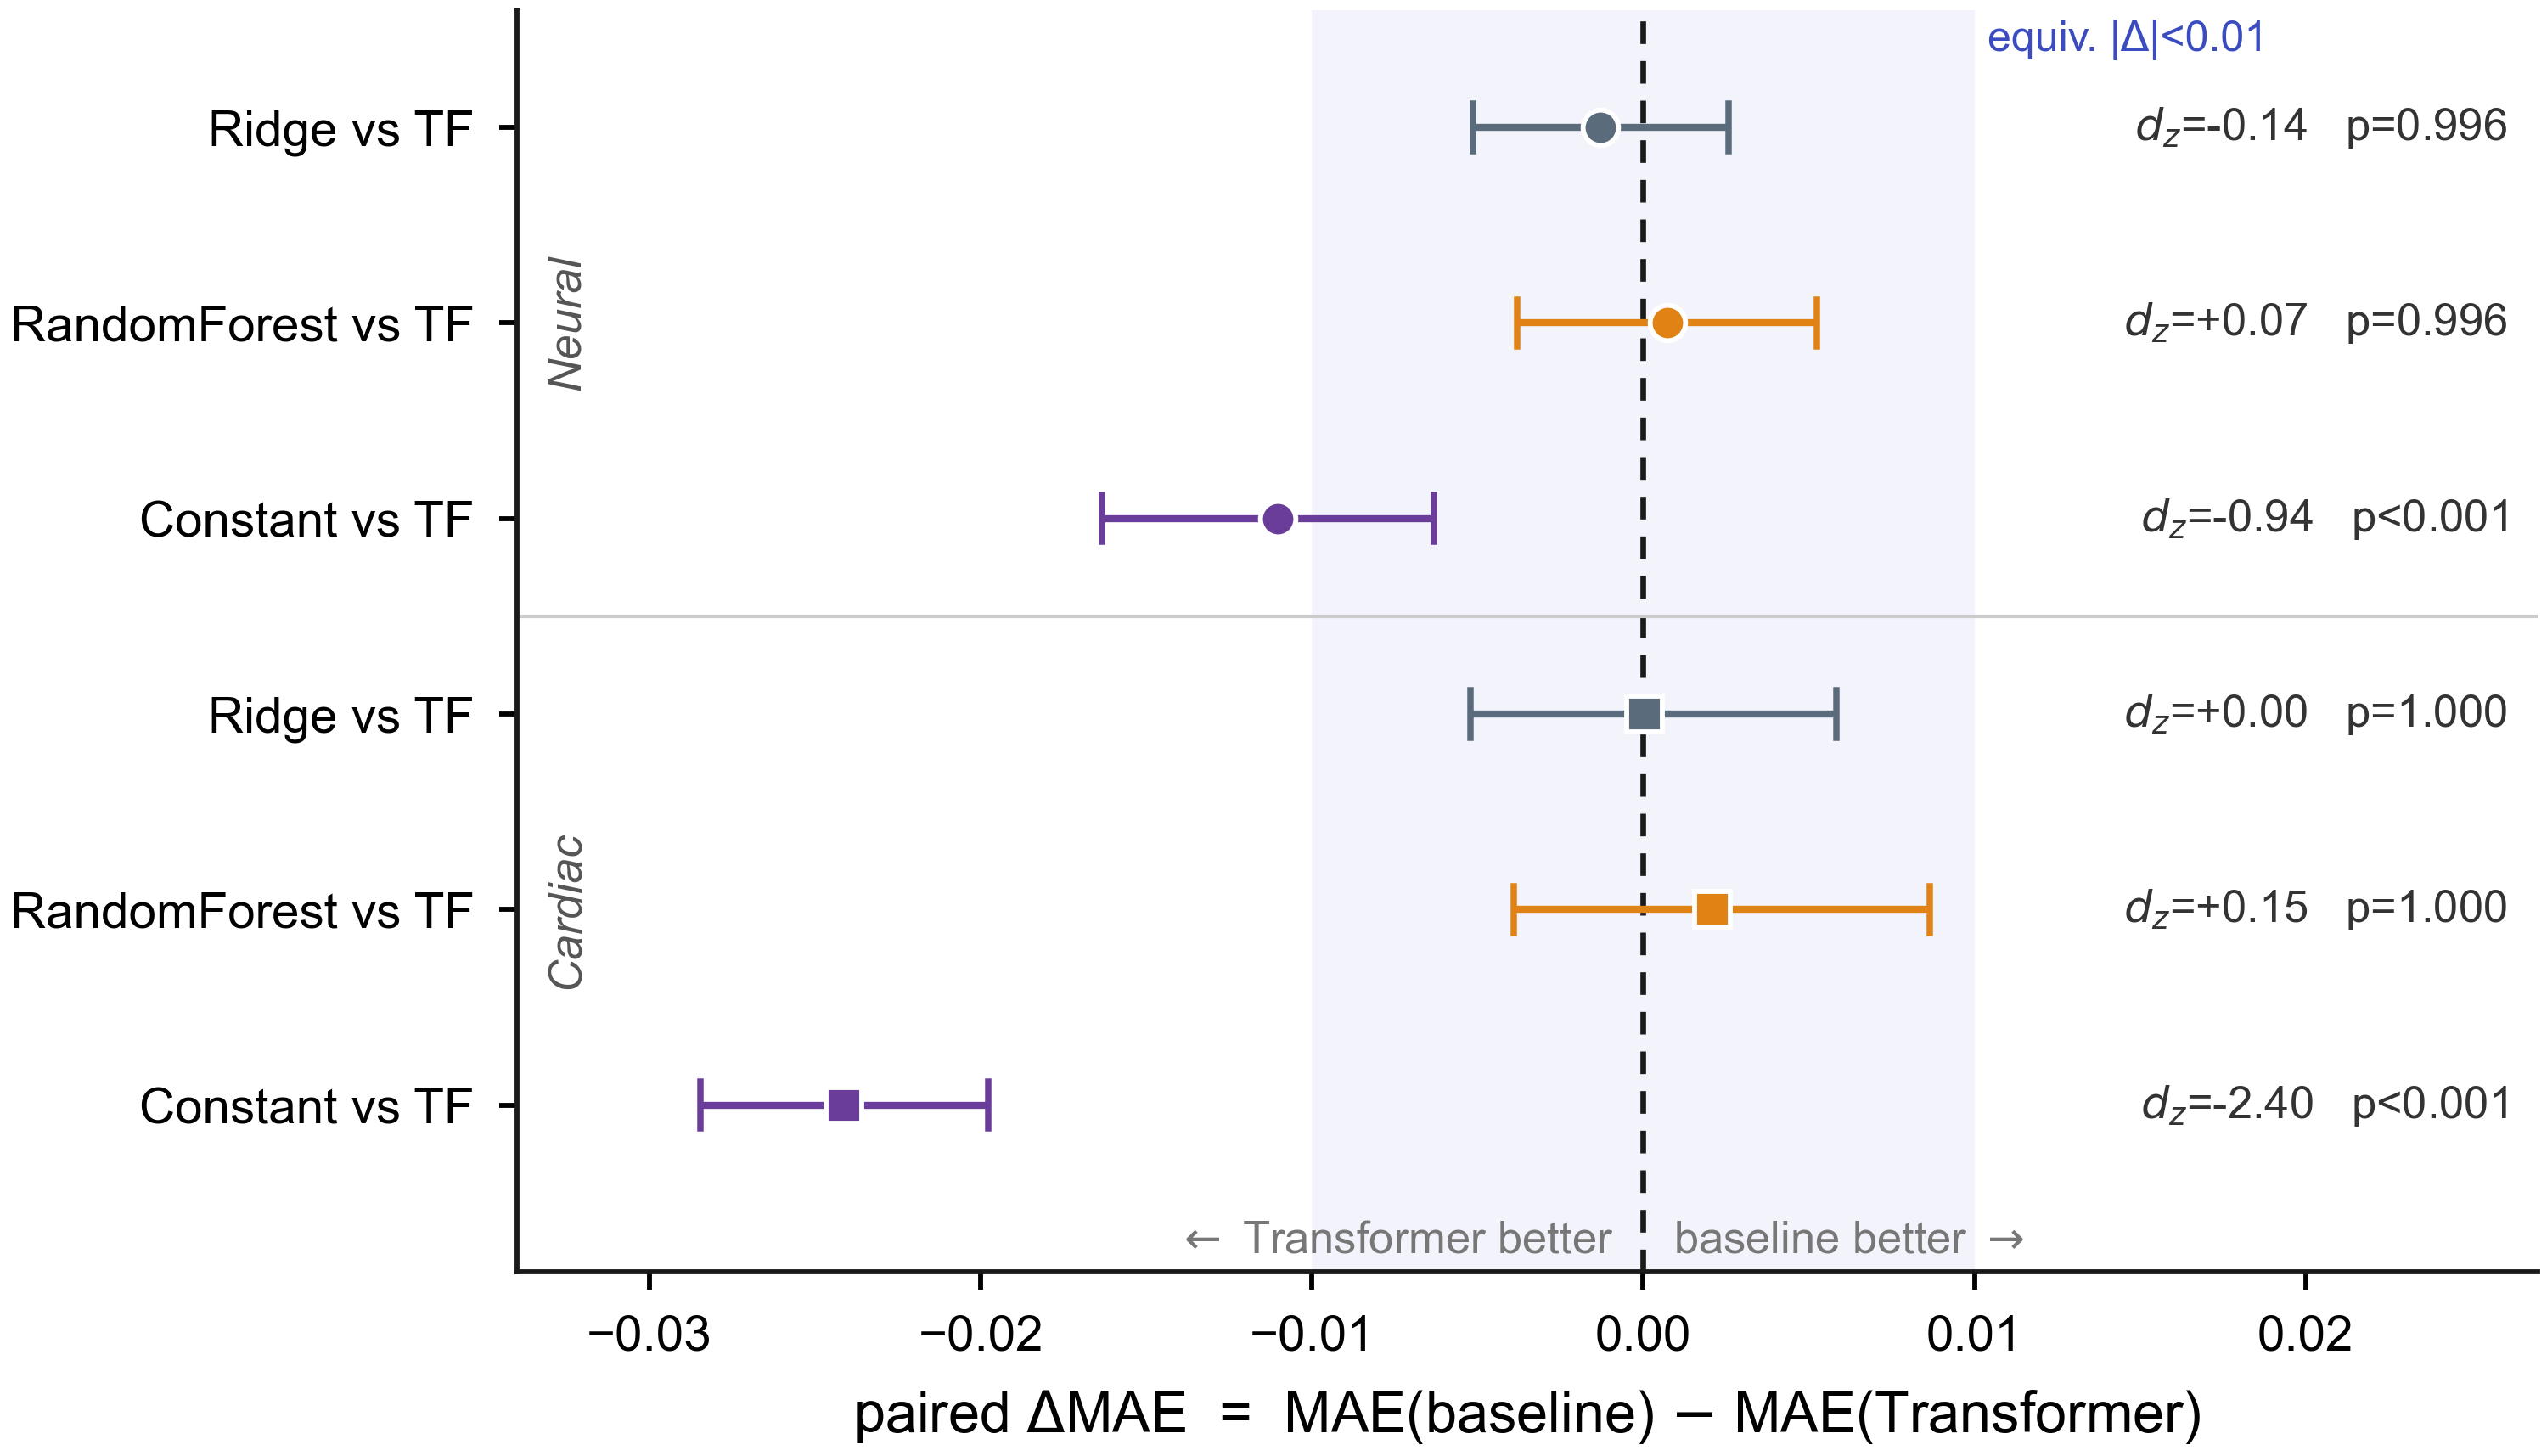
\includegraphics[width=\linewidth,height=0.78\textheight,keepaspectratio]{figures/fig2_forest.png}
\end{column}
\begin{column}{0.41\textwidth}
\small
\begin{itemize}
\setlength{\itemsep}{0.6em}
\item{} Transformer, Ridge, and random forest were equivalent
\item{} Constant median outperformed every trained model
\item{} Neural improvement: 6--7\%; cardiac improvement: 28--31\%
\end{itemize}
\end{column}
\end{columns}
\note{On independently paired data, the three trained models are statistically equivalent on both lineages. The constant training median is significantly better than all of them, with a 6--7\% lower error on the neural lineage and 28--31\% lower error on the cardiac lineage. The trained models behave like input-independent predictors.}
\end{frame}

\begin{frame}{Order Controls Do Not Prove Dependence Is Absent}
\begin{columns}[c]
\begin{column}{0.56\textwidth}
\centering
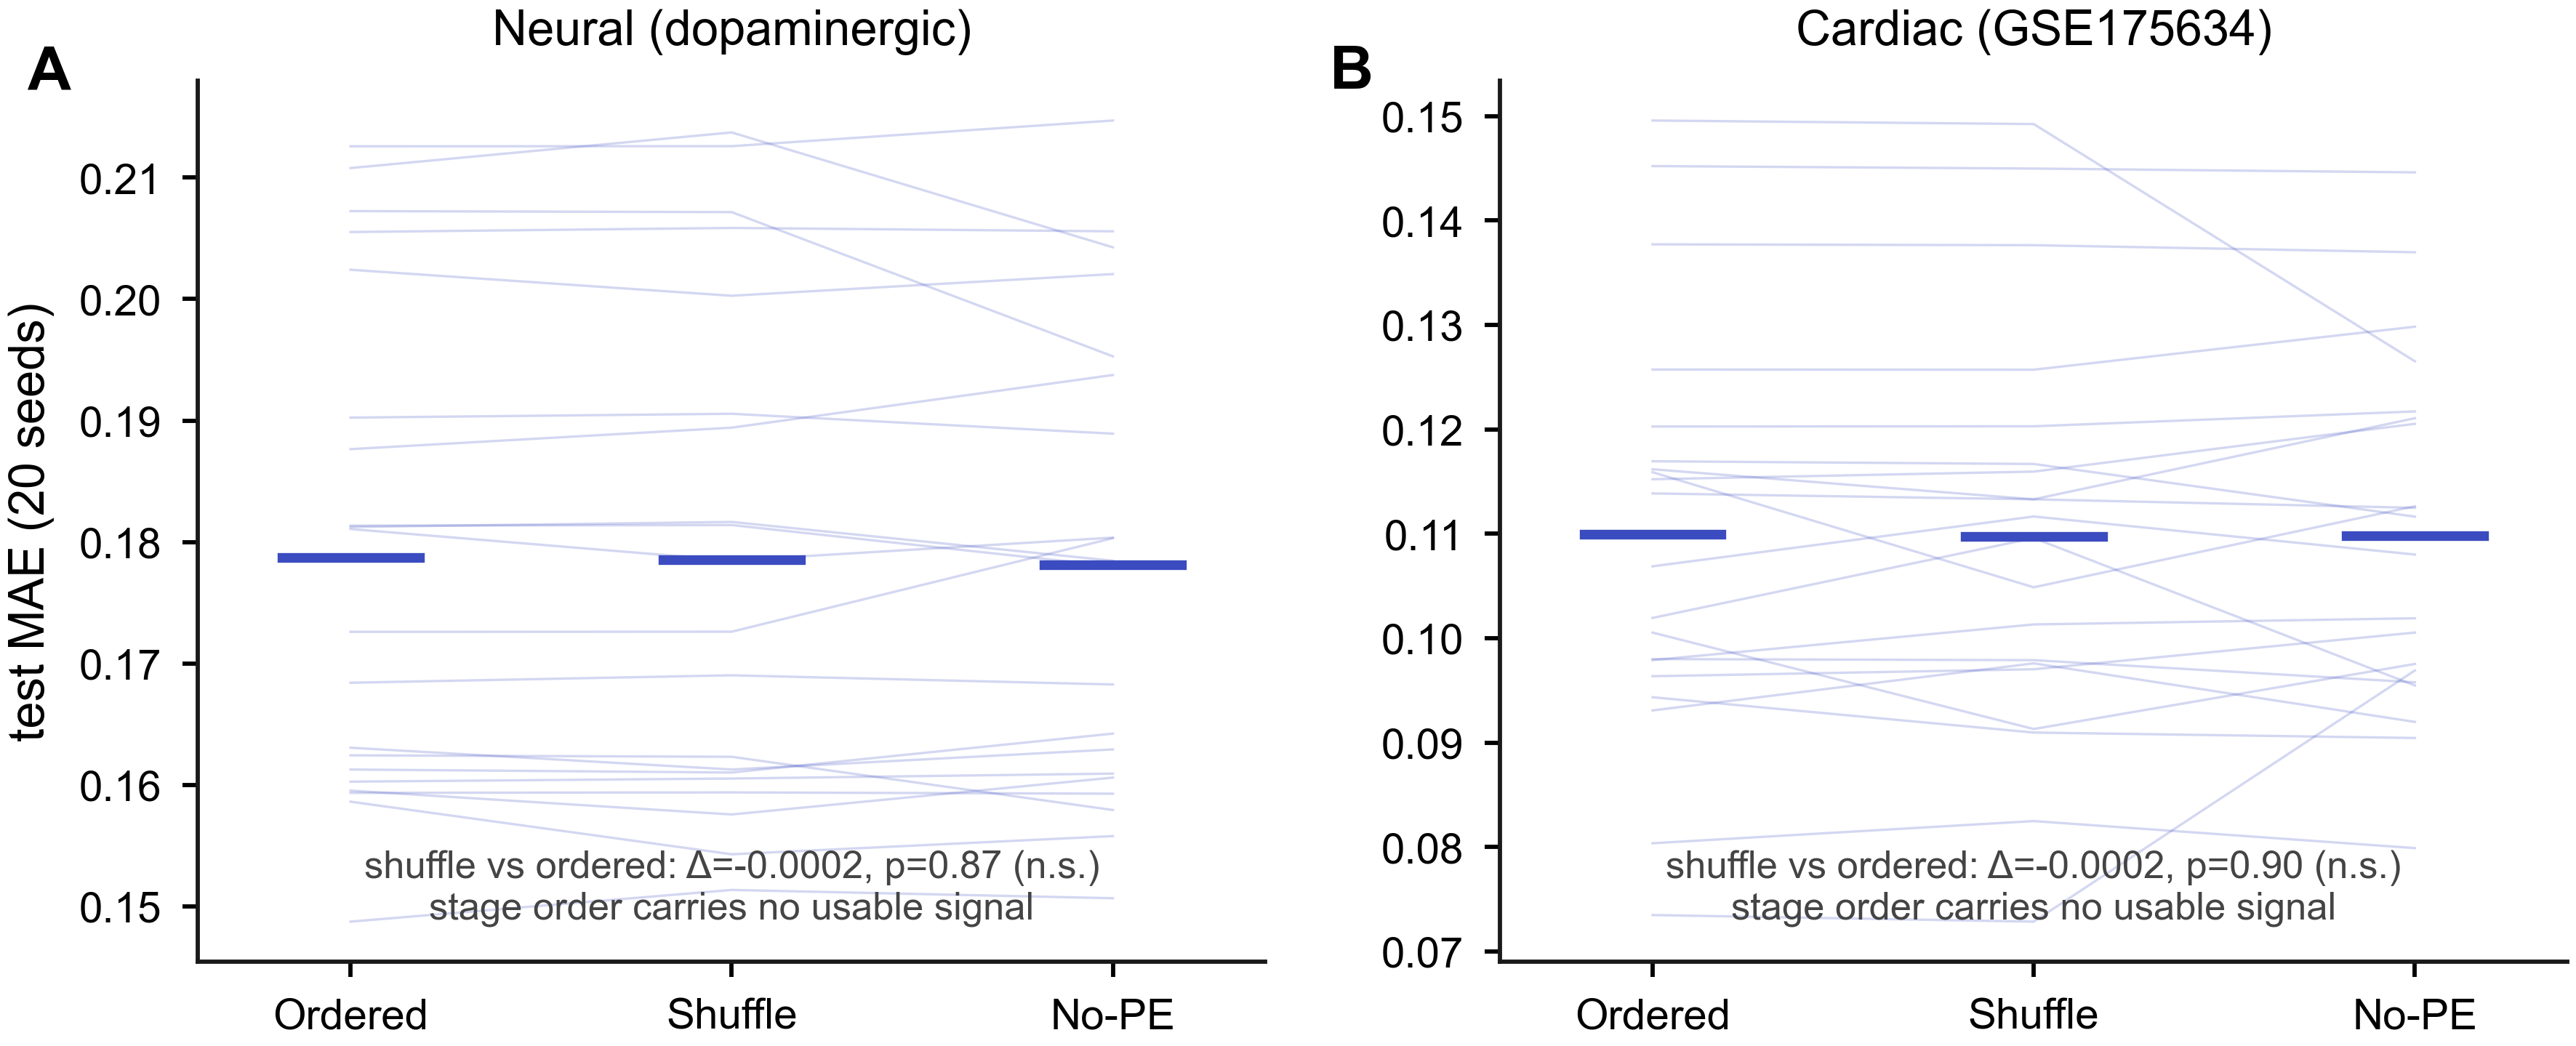
\includegraphics[width=\linewidth,height=0.78\textheight,keepaspectratio]{figures/fig4_temporal.png}
\end{column}
\begin{column}{0.41\textwidth}
\small
\begin{itemize}
\setlength{\itemsep}{0.6em}
\item{} Stage-order shuffle left accuracy unchanged
\item{} Removing positional encoding was equally inert
\item{} State values reveal stage identity
\item{} Shuffle controls require validation
\end{itemize}
\end{column}
\end{columns}
\note{Shuffling stage order or removing positional encoding did not change Transformer accuracy. That is consistent with the independent-pairing null, but it is not decisive by itself. In the positive control, stage identity could be inferred directly from state values, so the same shuffle remained insensitive despite genuine temporal dependence.}
\end{frame}

\begin{frame}{The Protocol Detects Dependence}
\begin{columns}[c]
\begin{column}{0.56\textwidth}
\centering
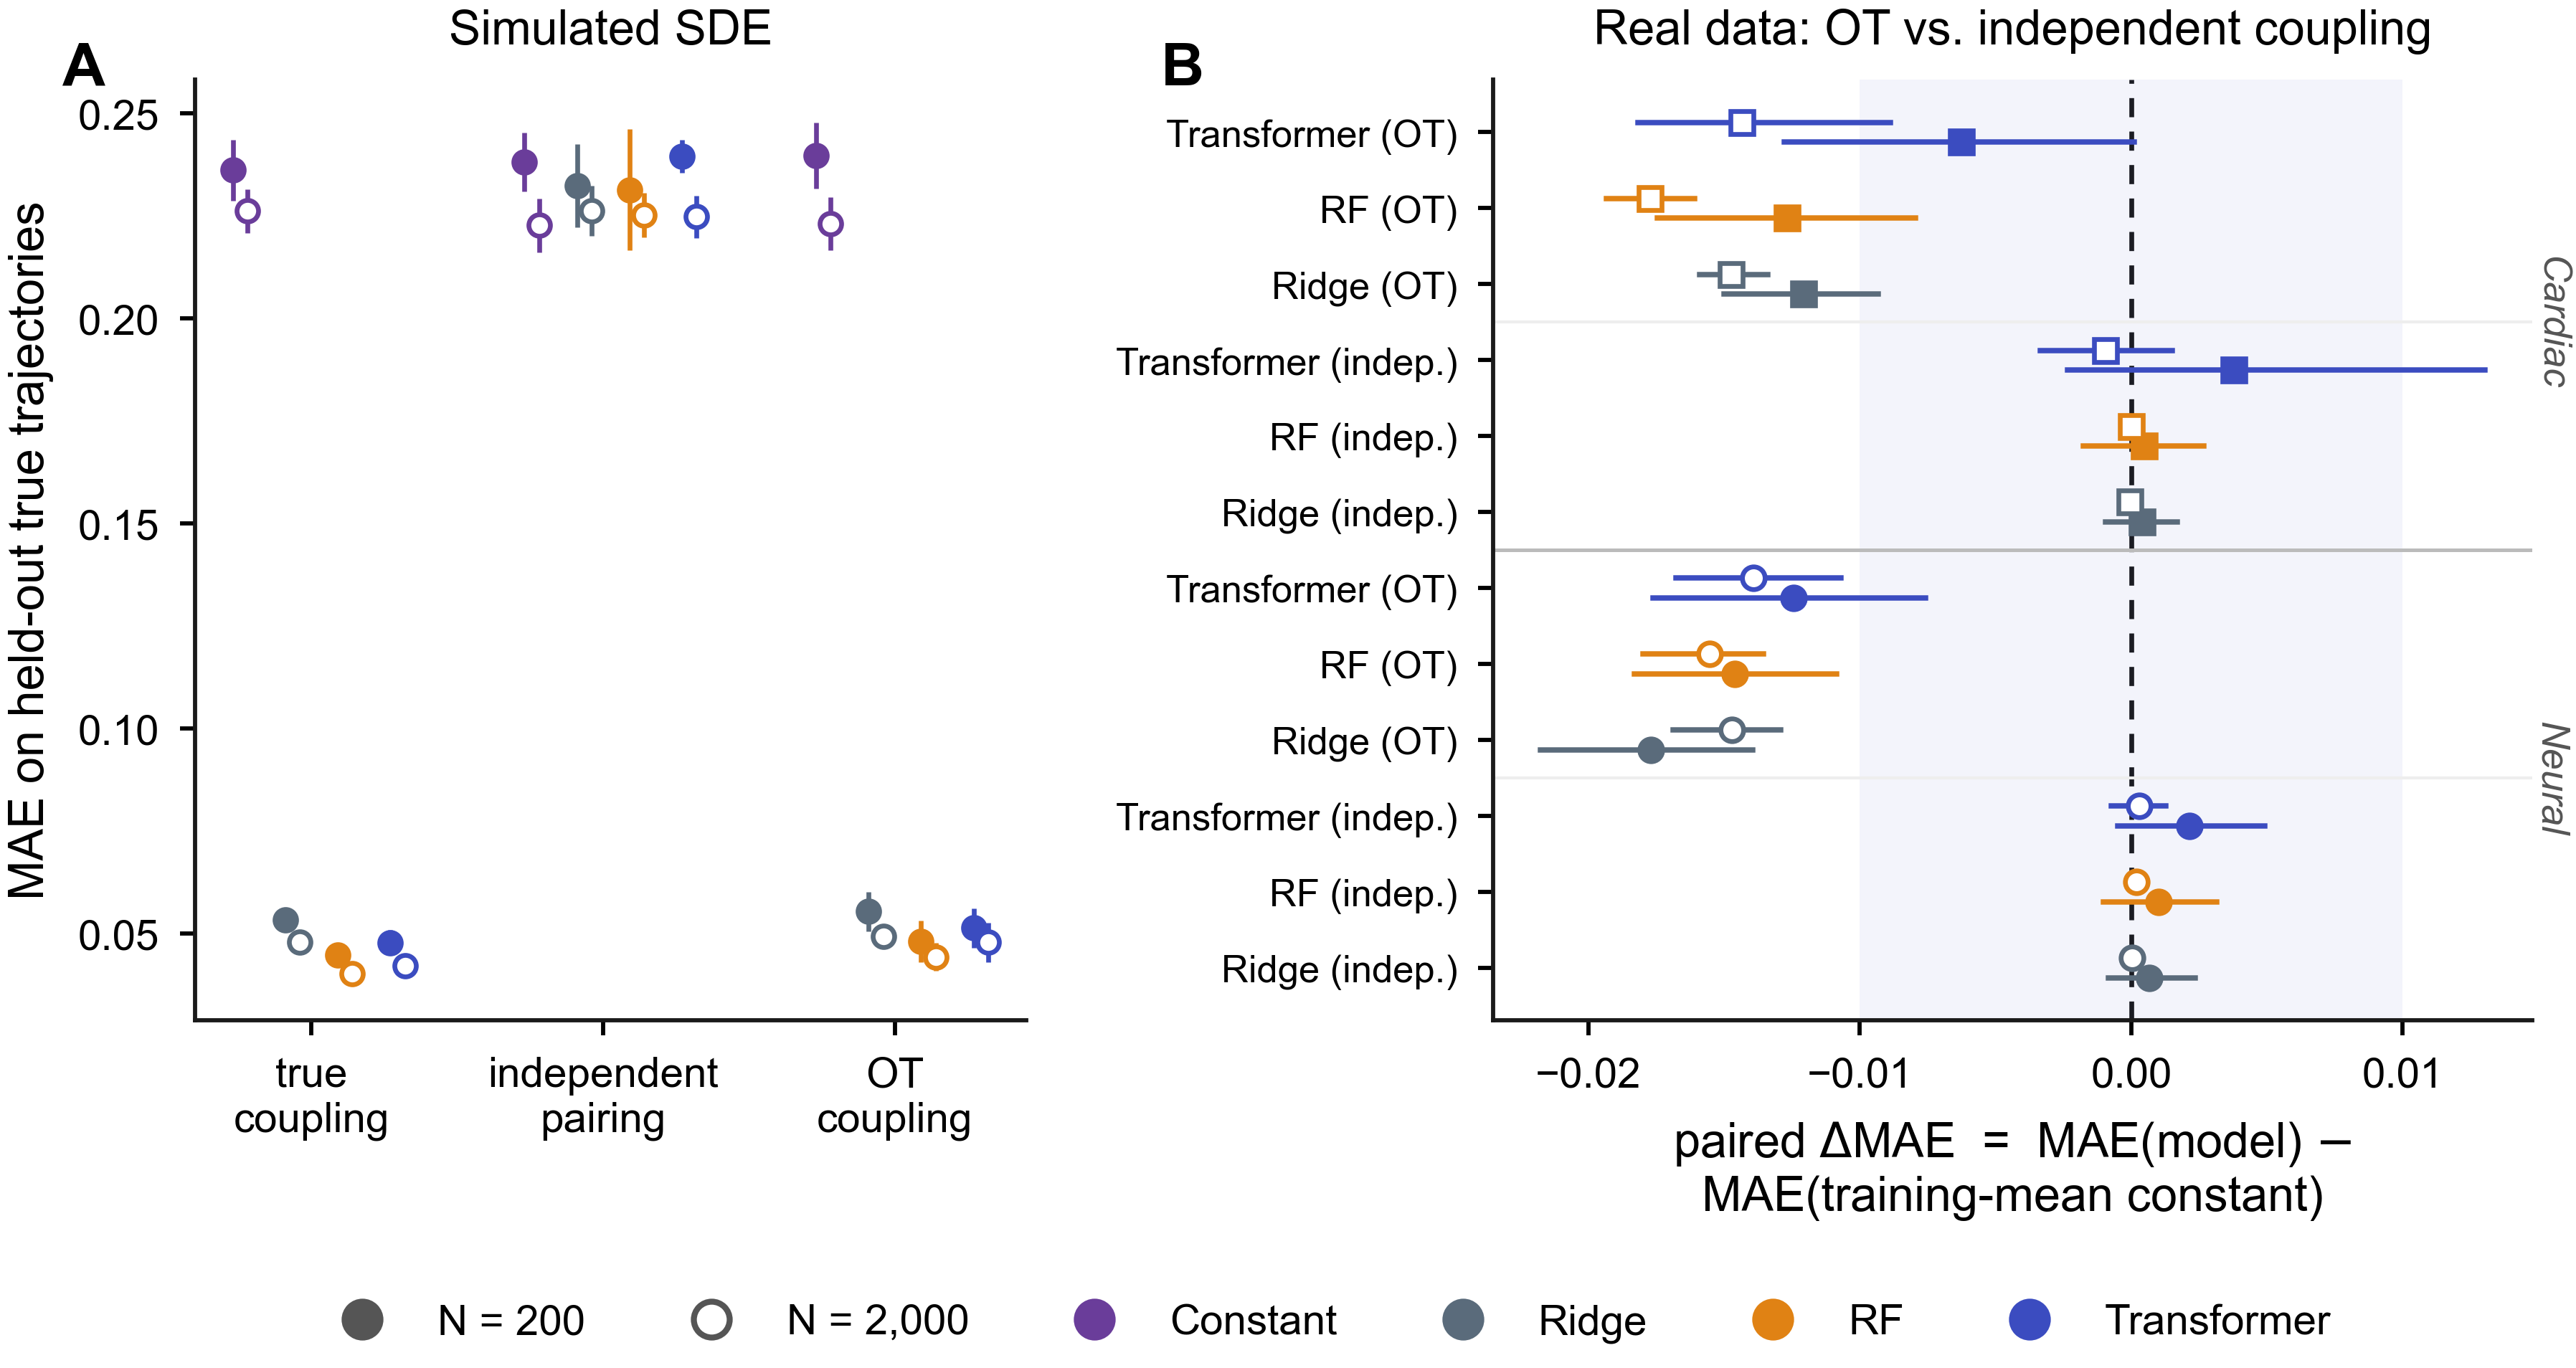
\includegraphics[width=\linewidth,height=0.78\textheight,keepaspectratio]{figures/fig7_positive.png}
\end{column}
\begin{column}{0.41\textwidth}
\small
\begin{itemize}
\setlength{\itemsep}{0.6em}
\item{} Simulation recovered genuinely recoverable dependence
\item{} OT coupling made real-data dependence detectable
\item{} Transformer never significantly beat random forest
\item{} OT dependence is induced, not proven biological
\end{itemize}
\end{column}
\end{columns}
\note{The positive controls show that the protocol can detect dependence when it is present. Simulation with known ground truth produced recoverable dependence, while OT-coupled real data allowed every model to beat the input-free baseline. This demonstrates sensitivity to coupling-induced information, not biological validation of the coupling.}
\end{frame}

\section{Takeaways}
\begin{frame}[plain]
\hxsectionslide{05}{Takeaways}
\end{frame}

\begin{frame}{Coupling, Not Capacity, Sets the Ceiling}
\begin{itemize}
\setlength{\itemsep}{0.6em}
\item{} Independent pairing yields a null by construction
\item{} Report coupling explicitly in every benchmark
\item{} Use metric-matched input-independent baselines
\item{} Evaluate leakage-safely across many seeds
\item{} Validate controls where dependence is known
\end{itemize}
\note{The central conclusion is that coupling determines what a forecasting benchmark can detect. Independent pairing creates a null, while OT coupling induces detectable dependence without proving biological correctness. Reliable benchmarks should state their coupling, include a metric-matched constant, use repeated leakage-safe evaluation, and validate controls in settings with known temporal dependence.}
\end{frame}

\begin{frame}[plain]
\hxclosingslide{Thank you}{Questions?}
\end{frame}

\end{document}
